
\renewcommand{\EntradaBibtex}{MarcoNuno_CongArbEsp_2021_10_02}

\begin{frame}{\citetitle{\EntradaBibtex}$^*$ (1)}
\begin{block}{Motivación} 
Durante la pandemia de COVID-19, muchos docentes se adaptaron  a nuevas formas para llevar a cabo sus actividades docentes. Uno de éstas es el pase de asistencia.
\begin{itemize}
\item Se desarrolló un aplicación de escritorio que analizara los archivos generados por un Plug-in de google para generar la asistencia con un click en las sesiones de Meet. 
\item Se analiza el horario del profesor y las horas de los archivos para cruzar a que clase pertenecen.
\item El profesor pasa asistencia con un click.
\item Estima porcentajes de asistencia de varias clases (y al interior de la misma clase).
%\item Genera un informe para establecer el \% de asistencia del estudiante.
\end{itemize}
\end{block} 
\footfullcite*{\EntradaBibtex}
\end{frame}


\begin{frame}{\citetitle{\EntradaBibtex} (2)}
%\begin{block}{Pantallas Principales} 

%\begin{columns}
% Column 1
%\column{.1\linewidth}
%\begin{center}
%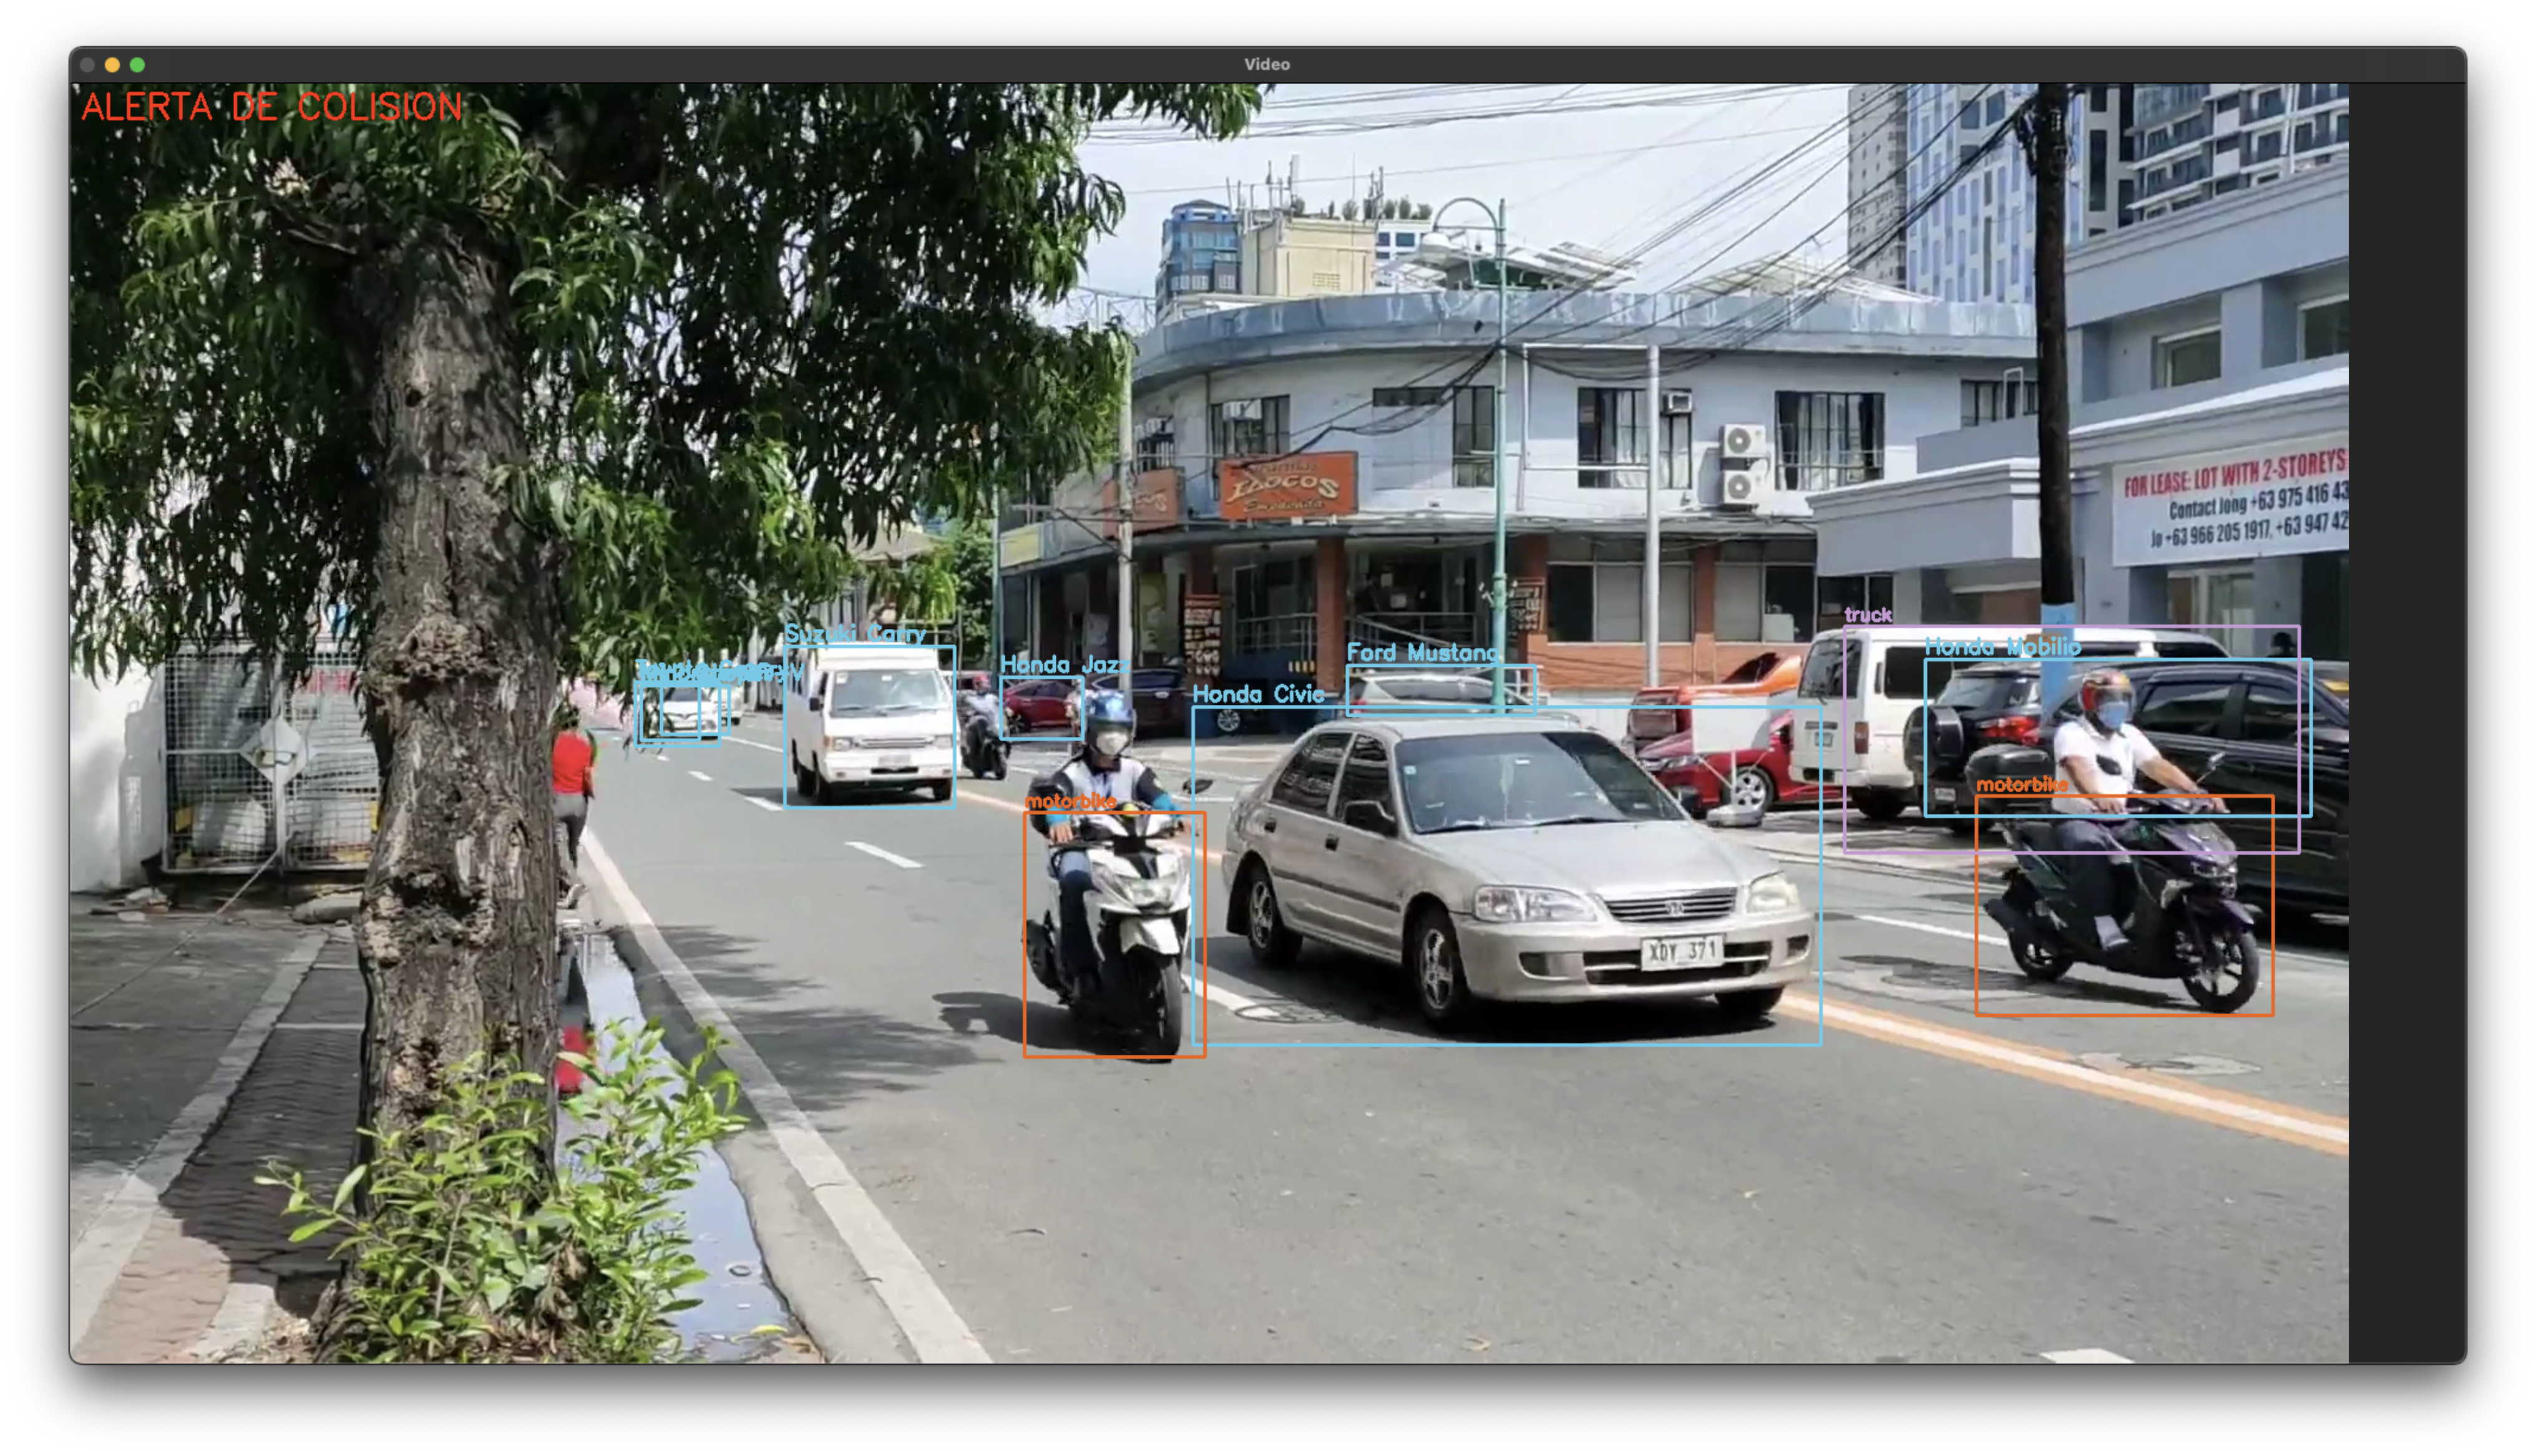
\includegraphics[width=0.85\linewidth]{2024_DetectorMotos/figs/resultados1.png}
%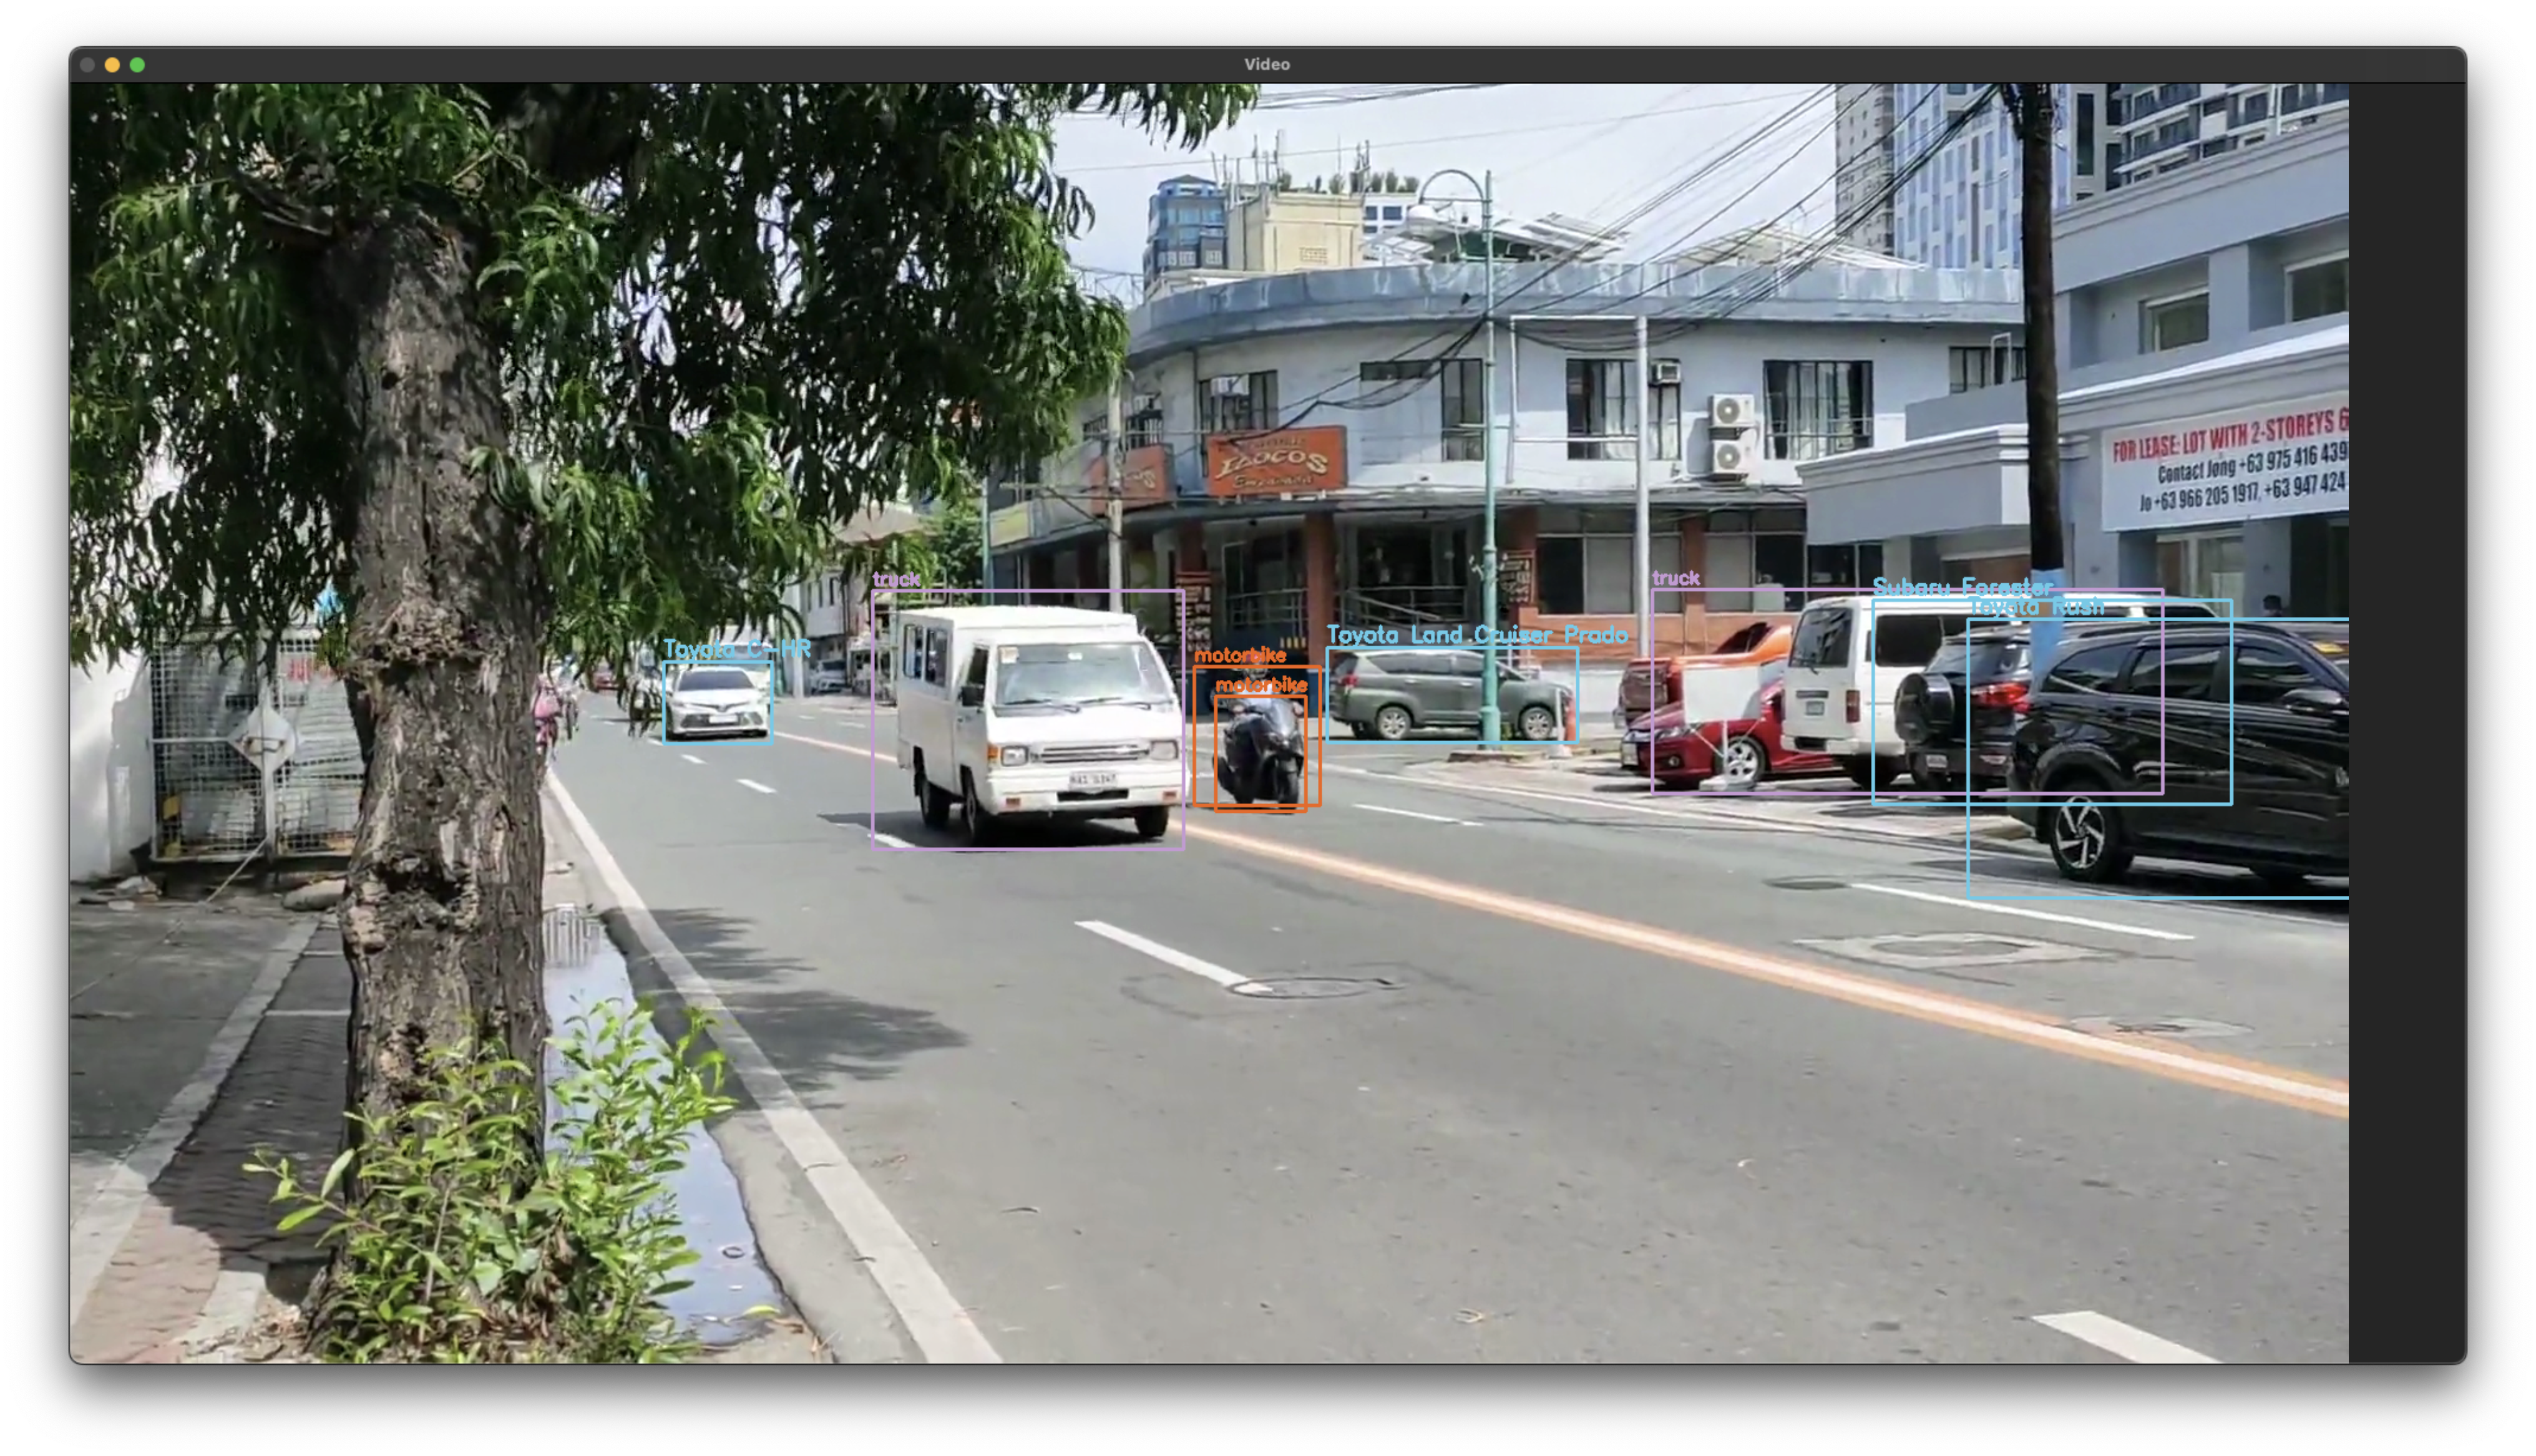
\includegraphics[width=0.85\linewidth]{2024_DetectorMotos/figs/resultados2.png}
%\end{center}
%\column{.9\linewidth}
El profesor puede establecer criterios para contabilizar asistencia
\begin{itemize}
\item Estudiante conectado en el 100\% de los eventos de asistencia para tal clase.
\item Estudiante conectado en el 70\% de los eventos de asistencia para tal clase.
\item Estudiante conectado en el 50\% de los eventos de asistencia para tal clase.
\end{itemize}
\begin{center}
	\begin{tabular}{cc}

%2021_ListaOnLine/figs/Informe2.png
		\includegraphics[width=0.40\linewidth]{2021_ListaOnLine/figs/Informe1.png} &
		\includegraphics[width=0.40\linewidth]{2021_ListaOnLine/figs/Informe2.png} \\
	\end{tabular}
\end{center}

%\end{columns}
\end{frame}



\begin{frame}{\citetitle{\EntradaBibtex} (3)}

El profesor puede establecer criterios para contabilizar asistencia
\begin{itemize}
\item Listado de los eventos de pase de lista por cada clase
\item Porcentaje de asistencia basada en los criterios para cada sesión del cuatrimestre
\end{itemize}
\begin{center}
	\begin{tabular}{cc}
		\includegraphics[width=0.40\linewidth]{2021_ListaOnLine/figs/Pases-608.png} &
		\includegraphics[width=0.40\linewidth]{2021_ListaOnLine/figs/Pases-608-Stacked.png} \\
	\end{tabular}
\end{center}

%\end{columns}
\end{frame}

